\documentclass[a4paper,12pt]{extarticle}
\usepackage{geometry}
\usepackage[T1]{fontenc}
\usepackage[utf8]{inputenc}
\usepackage[english,russian]{babel}
\usepackage{amsmath}
\usepackage{amsthm}
\usepackage{amssymb}
\usepackage{fancyhdr}
\usepackage{setspace}
\usepackage{graphicx}
\usepackage{colortbl}
\usepackage{tikz}
\usepackage{pgf}
\usepackage{subcaption}
\usepackage{listings}
\usepackage{indentfirst}
\usepackage[
backend=biber,
style=numeric,
maxbibnames=99
]{biblatex}
\addbibresource{refs.bib}
\usepackage[colorlinks,citecolor=blue,linkcolor=blue,bookmarks=false,hypertexnames=true, urlcolor=blue]{hyperref} 
\usepackage{indentfirst}
\usepackage{mathtools}
\usepackage{booktabs}
\usepackage[flushleft]{threeparttable}
\usepackage{tablefootnote}

\usepackage{chngcntr} % нумерация графиков и таблиц по секциям
\counterwithin{table}{section}
\counterwithin{figure}{section}

\graphicspath{{graphics/}}%путь к рисункам

\makeatletter
% \renewcommand{\@biblabel}[1]{#1.} % Заменяем библиографию с квадратных скобок на точку:
\makeatother

\geometry{left=2.5cm}% левое поле
\geometry{right=1.0cm}% правое поле
\geometry{top=2.0cm}% верхнее поле
\geometry{bottom=2.0cm}% нижнее поле
\setlength{\parindent}{1.25cm}
\renewcommand{\baselinestretch}{1.5} % междустрочный интервал


\newcommand{\bibref}[3]{\hyperlink{#1}{#2 (#3)}} % biblabel, authors, year
\addto\captionsrussian{\def\refname{Список литературы (или источников)}} 

\renewcommand{\theenumi}{\arabic{enumi}}% Меняем везде перечисления на цифра.цифра
\renewcommand{\labelenumi}{\arabic{enumi}}% Меняем везде перечисления на цифра.цифра
\renewcommand{\theenumii}{.\arabic{enumii}}% Меняем везде перечисления на цифра.цифра
\renewcommand{\labelenumii}{\arabic{enumi}.\arabic{enumii}.}% Меняем везде перечисления на цифра.цифра
\renewcommand{\theenumiii}{.\arabic{enumiii}}% Меняем везде перечисления на цифра.цифра
\renewcommand{\labelenumiii}{\arabic{enumi}.\arabic{enumii}.\arabic{enumiii}.}% Меняем везде перечисления на цифра.цифра

\lstset { % for c++ code field
    language=C++,
    backgroundcolor=\color{black!5}, % set backgroundcolor
    basicstyle=\footnotesize,% basic font setting
}

\begin{document}
% \begin{titlepage}
\newpage

{\setstretch{1.0}
\begin{center}
ПРАВИТЕЛЬСТВО РОССИЙСКОЙ ФЕДЕРАЦИИ\\
ФГАОУ ВО НАЦИОНАЛЬНЫЙ ИССЛЕДОВАТЕЛЬСКИЙ УНИВЕРСИТЕТ\\
«ВЫСШАЯ ШКОЛА ЭКОНОМИКИ»
\\
\bigskip
Факультет компьютерных наук\\
Образовательная программа «Прикладная математика и информатика»
\end{center}
}

\vspace{2em}
УДК 
\vspace{5em}

\begin{center}
%Выберите какой у вас проект
{\bf Отчет о программном проекте на тему:}\\
%{\bf Отчет о программном проекте на тему:}\\
{\bf Приложение для визуализации Персистентной очереди}
\end{center}

\vspace{2em}

{\bf Выполнил: \vspace{2mm}}

{\setstretch{1.0}
\begin{tabular}{l@{\hskip 1.5cm}c@{\hskip 1.5cm}c}
студент группы БПМИ216 & & \\
Фаткуллин Фёдор Алексеевич & \rule{3.5cm}{0.15mm}  &  \rule{3.5cm}{0.15mm} \vspace{-2mm} \\
 & \tiny{(подпись)}  & \tiny{(дата)} \\
\end{tabular}}

\vspace{1em}
{\bf Принял руководитель проекта: \vspace{2mm}}

{\setstretch{1.0}
\begin{tabular}{l@{\hskip 1.5cm}l}
Самоненко Илья Юрьевич\\
Научный сотрудник\\
Факультета компьютерных наук НИУ ВШЭ \vspace{10mm}\\
\rule{4cm}{0.15mm}  &  \rule{4cm}{0.15mm} \vspace{-2mm}\\
{\hskip 1.5cm}\tiny{(подпись)} & {\hskip 1.5cm}\tiny{(дата)} \\
\end{tabular}}

\vspace{\fill}

\begin{center}
Москва 2023
\end{center}

\end{titlepage}% это титульный лист - выберите подходящий вам из имеющихся в проекте вариантов
\newpage
\setcounter{page}{2}

{
	\hypersetup{linkcolor=black}
	\tableofcontents
}

\newpage

\newpage
\section*{Аннотация}
Для изучения алгоритмов и структур данных часто не хватает инструмента, который бы давал возможность детально разобраться в алгоритме, не полагаясь исключительно на его техническое описание словами.\par
Мной была выбрана структура данных Персистентная очередь, которая широко применяется и известна в целом, но имеет сложные алгоритмы внутренней работы. Основная цель данной работы это предоставление понятного алгоритма и его визуальная реализация, для дополнительной показательности. С этой целью было разработано веб-приложение, которое отвечает основным требованиям к процессам визуализации и может применяться для наглядного изучения этой структуры данных.

\addcontentsline{toc}{section}{Аннотация}

\section*{Ключевые слова}
Персистентная очередь, структура данных, визуализация алгоритма, алгоритм на графах, алгоритмическая оптимизация, пошаговость, односвязные списки.
\pagebreak

\section{Введение}
Предмет «Алгоритмы и структуры данных» по праву считается одним из основополагающих в изучении компьютерных наук. Но для многих студентов он становится одним из самых сложных в прохождении. Большинство алгоритмов не имеют физического представления и являются абстракциями, что вызывает определенные трудности у студентов. От понимания студентом тех или иных алгоритмов зависит его общее представление о возможностях их применения в решениях реальных прикладных задач. Для облегчения учебного процесса и более лучшего понимания преподаватели прибегают к визуализации, чтобы показать пошаговую работу алгоритмов в конкретных случаях.\par
Однако, не все алгоритмы можно наглядно изобразить на доске. Особенные трудности представляют алгоритмы на графах. Их сложно рисовать, на каждый шаг может уходить слишком много времени. Доска ограничена в размерах и через некоторое время быстро заполняется. Нельзя вернуться к предыдущему шагу и посмотреть на него снова. А самое главное, если детально не запомнить подробности работы, то нельзя самому воспроизвести его работу после занятия. При воспроизведении механизма работы алгоритма нельзя исключать и  вероятность случайной ошибки как студента, так и преподавателя.\par
Все вышеперечисленные проблемы можно решить с помощью современных решений — визуализации работы алгоритма в веб-приложении. Такой подход исключает человеческий фактор ошибки, рабочее пространство не ограничено пределами доски, а визуализация будет выглядеть четко и понятно. Все шаги выполнения комментируются, давая студенту возможность поэксперементировать самому с алгоритмом и посмотреть на его работу вне учебных занятий. Также, открываются новые возможности для рассмотрения работы на больших массивах данных. Например, построить граф на несколько сотен вершин, провести аналитику над ним и узнать общую эффективность алгоритма.\par
По этой причине визуализации алгоритмов будут всегда актуальны для обучения. С этим связан мой выбор реализовать веб-приложение по визуализации работы такой структуры данных, как персистентная очередь. Эта структура данных является одновременно прикладной в решении реальных задач и сложной в освоении из-за неочевидных алгоритмов взаимодействия с ней.\par
По проведенным мной исследованиям доступных решений, на данный момент не существует ни одной визуализации данной структуры данных в открытом доступе для пользователей. Данный факт увеличивает актуальность разработки такого веб-приложения, поскольку это даст возможность изучать методы работы с данной структурой данных, что невозможно сделать с доступными в этот момент инструментами визуализации алгоритмов.\\

\section{Постановка задачи}
Необходимо разработать веб-приложение для визуализации Персистентной очереди, к которому предлагаются следующие требования:
\begin{itemize}
    \item Веб-приложение должно в явном виде демонстрировать структуру графа, его связи, обозначения и состояние. Все вершины должны быть подписаны.
    \item Должна присутствовать возможность масштабирования изображения графа, его перемещения.
    \item Пошаговость визуализации должна контролироваться пользователем.
    \item Должна быть возможность откатов назад, для повторений шагов.
    \item Все шаги должны быть снабжены описанием того, что происходит.
    \item У веб-приложения должен существовать дополнительный интерфейс взаимодествия, помимо выполнения простых операций.
\end{itemize}
С этой целью основная задача разбивается на две основных подзадачи:
\begin{enumerate}
    \item Выбор алгоритма взаимодействия с Персистентной очередью и способ ее хранения.
    \item Разработка непосредственно веб-приложения, основанного на работе по выбранному ранее алгоритму.
\end{enumerate}

\section{Разработка алгоритма}
\subsection{Выбор алгоритма}
После ознакомления с существующими распространенными вариантами реализации Персистентной очереди, можно заметить что почти подавляющее большинство - алгоритмы на разном количестве стеков. Например, на 4~\cite{codeforces} или на 6~\cite{neerc-ifmo}(с возможной оптимизацией до 5). Также, существуют реализации на персистентном дереве отрезков и на персистентном декартовом дереве по неявному ключу.\par
Однако, по моему мнению, такие способы реализации сложны и требуют глубокого понимания, что мне не подходит. По этой причине, мной был разработан алгоритм на двух деревьях (на основе предложенного здесь~\cite{habr}), который не только интуитивно понятнее, но и гораздо нагляднее ранее упомянутых.

\subsection{Терминология}
\noindentДалее по тексту будут применяться следующие слова, с измененным смыслом:
\begin{itemize}
    \item Список — односвязный список в традиционном программном понимании.
    \item Очередь — то же, что и список.
    \item Сын — следующий по списку объект.
    \item Версия — объект, который хранит в себе данные об определённой очереди.
    \item Вершина - объект, содержащий информацию о текущем элементе и указатель на Сына.
    \item Целевая вершина — то же, что и вершина.
    \item Основное дерево — дерево (лес), представляющее собой непосредственно различные вариации очереди, состоит из Вершин.
    \item Вспомогательная вершина — объект, содержащий в себе указатель на Целевую вершину и указатель на Сына.
    \item Вспомогательное дерево — дерево (лес), представляющее собой вспомогательные списки для выполнения операций над очередями, состоит из Вспомогательных вершин.
    \item Хвост — последняя вершина в списке (она не содержится ни у кого в качестве сына).
    \item Ведущая вершина — то же, что и хвост.
    \item Голова — первая вершина списка (у нее нет сына).
    \item Промежуточная вершина — вершина, не являющаяся ни головой, ни хвостом.
\end{itemize}

\subsection{Основная идея и описание}
Везде в алгоритме объекты и элементы иммутабельны — после своего создания и завершения выполнения очередной операции становятся неизменяемыми.\par
Для хранения очереди воспользуемся Основным деревом. Эта структура используется и при построении персистентных стеков, где в каждой вершине записан непосредственно сам элемент и указатель на лежащий под ним (в терминологии очереди — "предшествующий ему"). Создадим пустой список объектов Версий — каждый такой объект представляет собой конкретное состояние очереди в определенный момент. Для этого, Версии достаточно состоять из 2 указателей — на Хвост и Голову очереди.\\
\begin{figure}[h!]
	\centering
	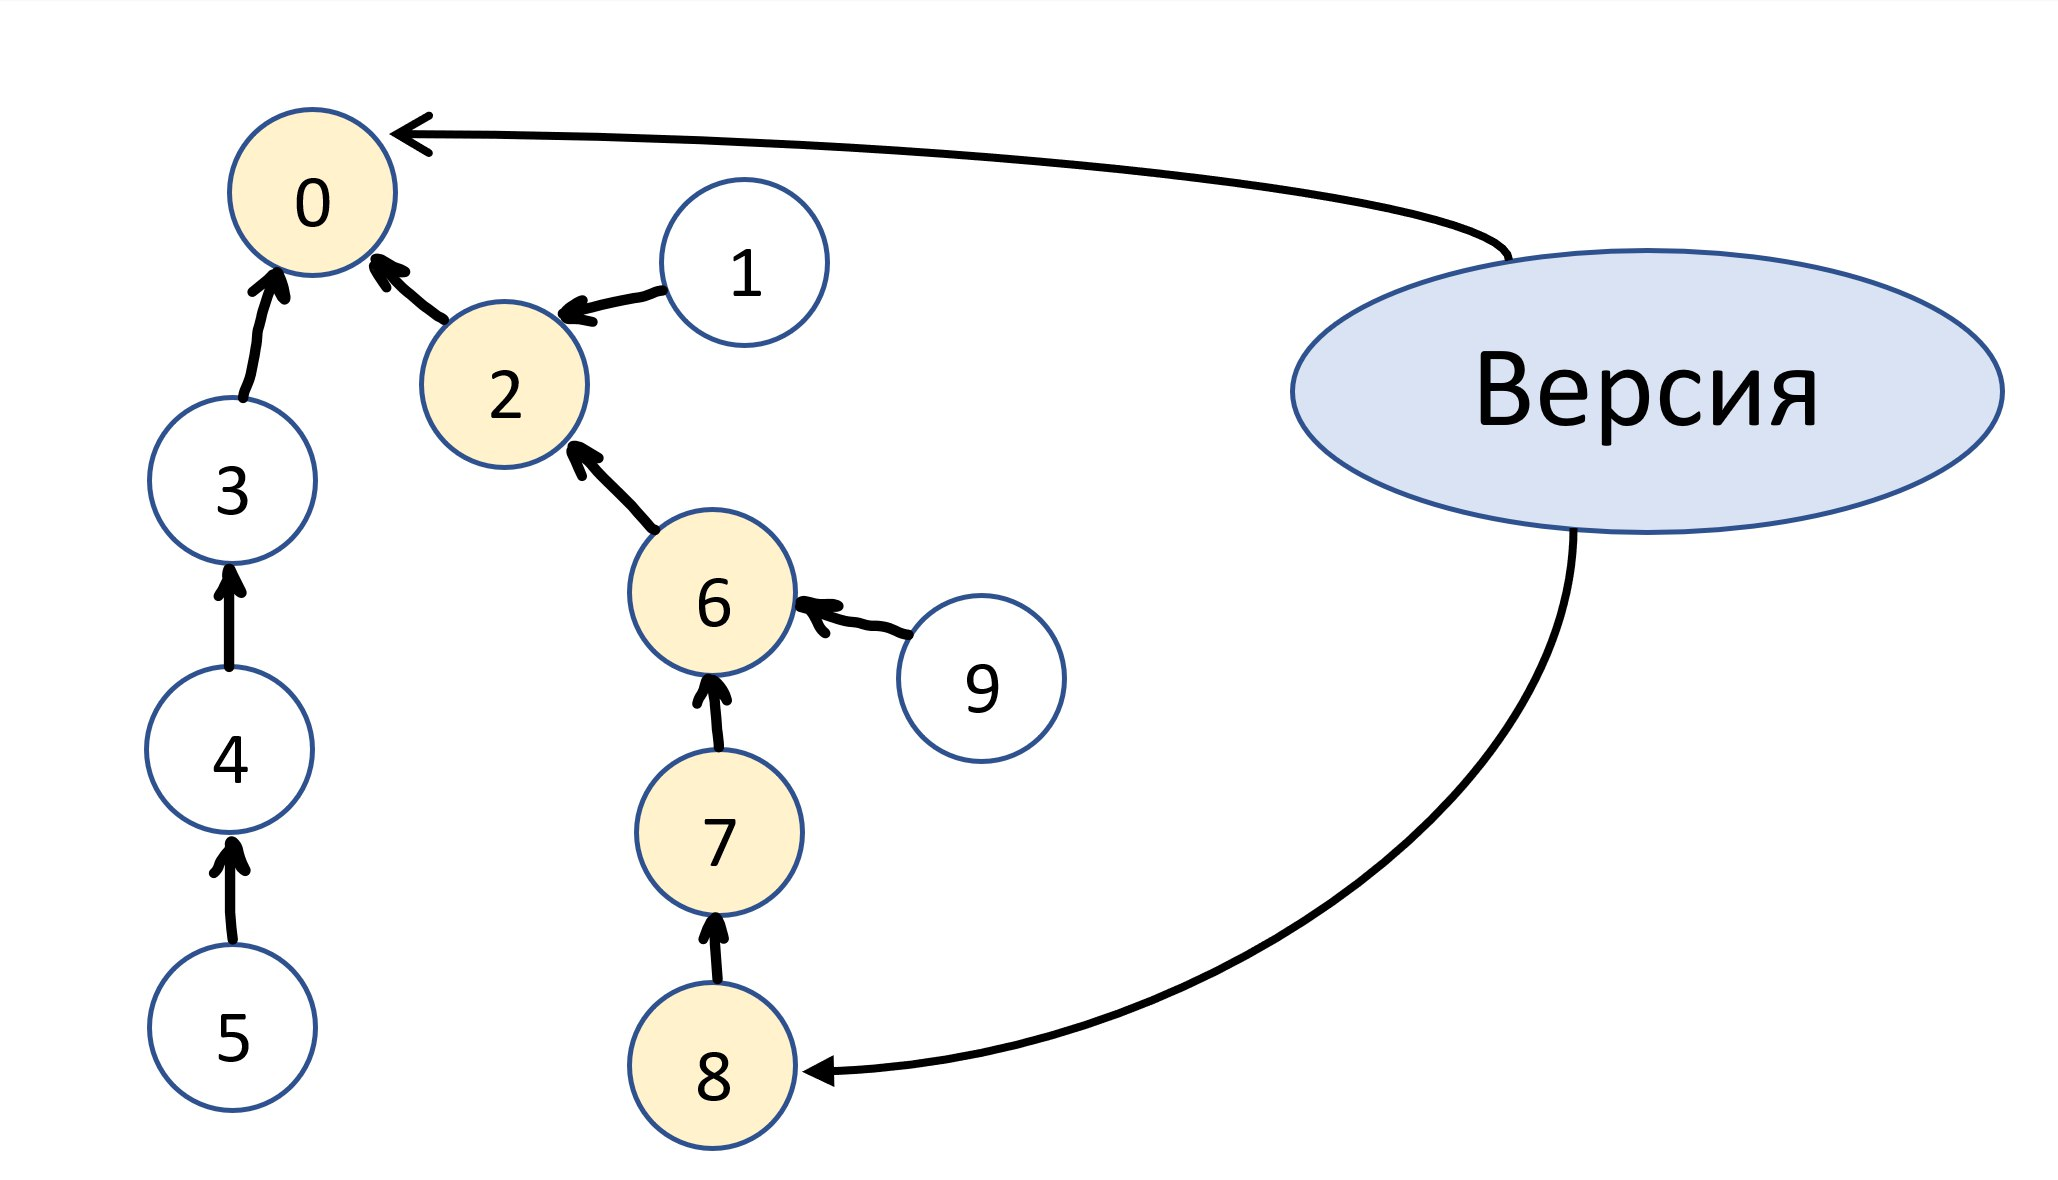
\includegraphics[width=0.6\textwidth]{content/1_img.jpg}
	\caption{Два указателя могут полностью охарактеризовать очередь}
	\label{version}
\end{figure}\par
Нумерацию этого списка начнем с 0, добавив в список исходную Версию, заполненную так, чтобы она показывала пустую очередь — отсутствие каких либо элементов на начало работы алгоритма. Тогда, при работе можно обратиться к любой Версии, зная ее уникальный порядковый номер. Любая операция над нашей структурой данных будет создавать и добавлять в конец списка новую Версию, показывающую состояние очереди на момент завершения операции.\\
Зная номер существующей Версии, можно совершить над ней две основные операции:
\begin{itemize}
    \item Удалить первый элемент из очереди.
    \item Добавить новый элемент в конец очереди.
\end{itemize}\par
Каждая из операций видоизменяет Основное дерево, при этом изменения не затрагивают элементы самой очереди и выбранную Версию. Таким образом, исходная очередь все равно доступна и продолжает храниться в соответствующей ей Версии.\par
Для реализации операции Добавления вершины в очередь такого интерфейса уже достаточно — каждая такая операция будет добавлять в Основное дерево новую вершину, подвязанную к хвостовой (ее мы можем узнать из указателей исходной Версии) и добавлять в список Версий копию исходной, с измененным указателем на хвостовую вершину.\\
\begin{figure}[h!]
	\centering
	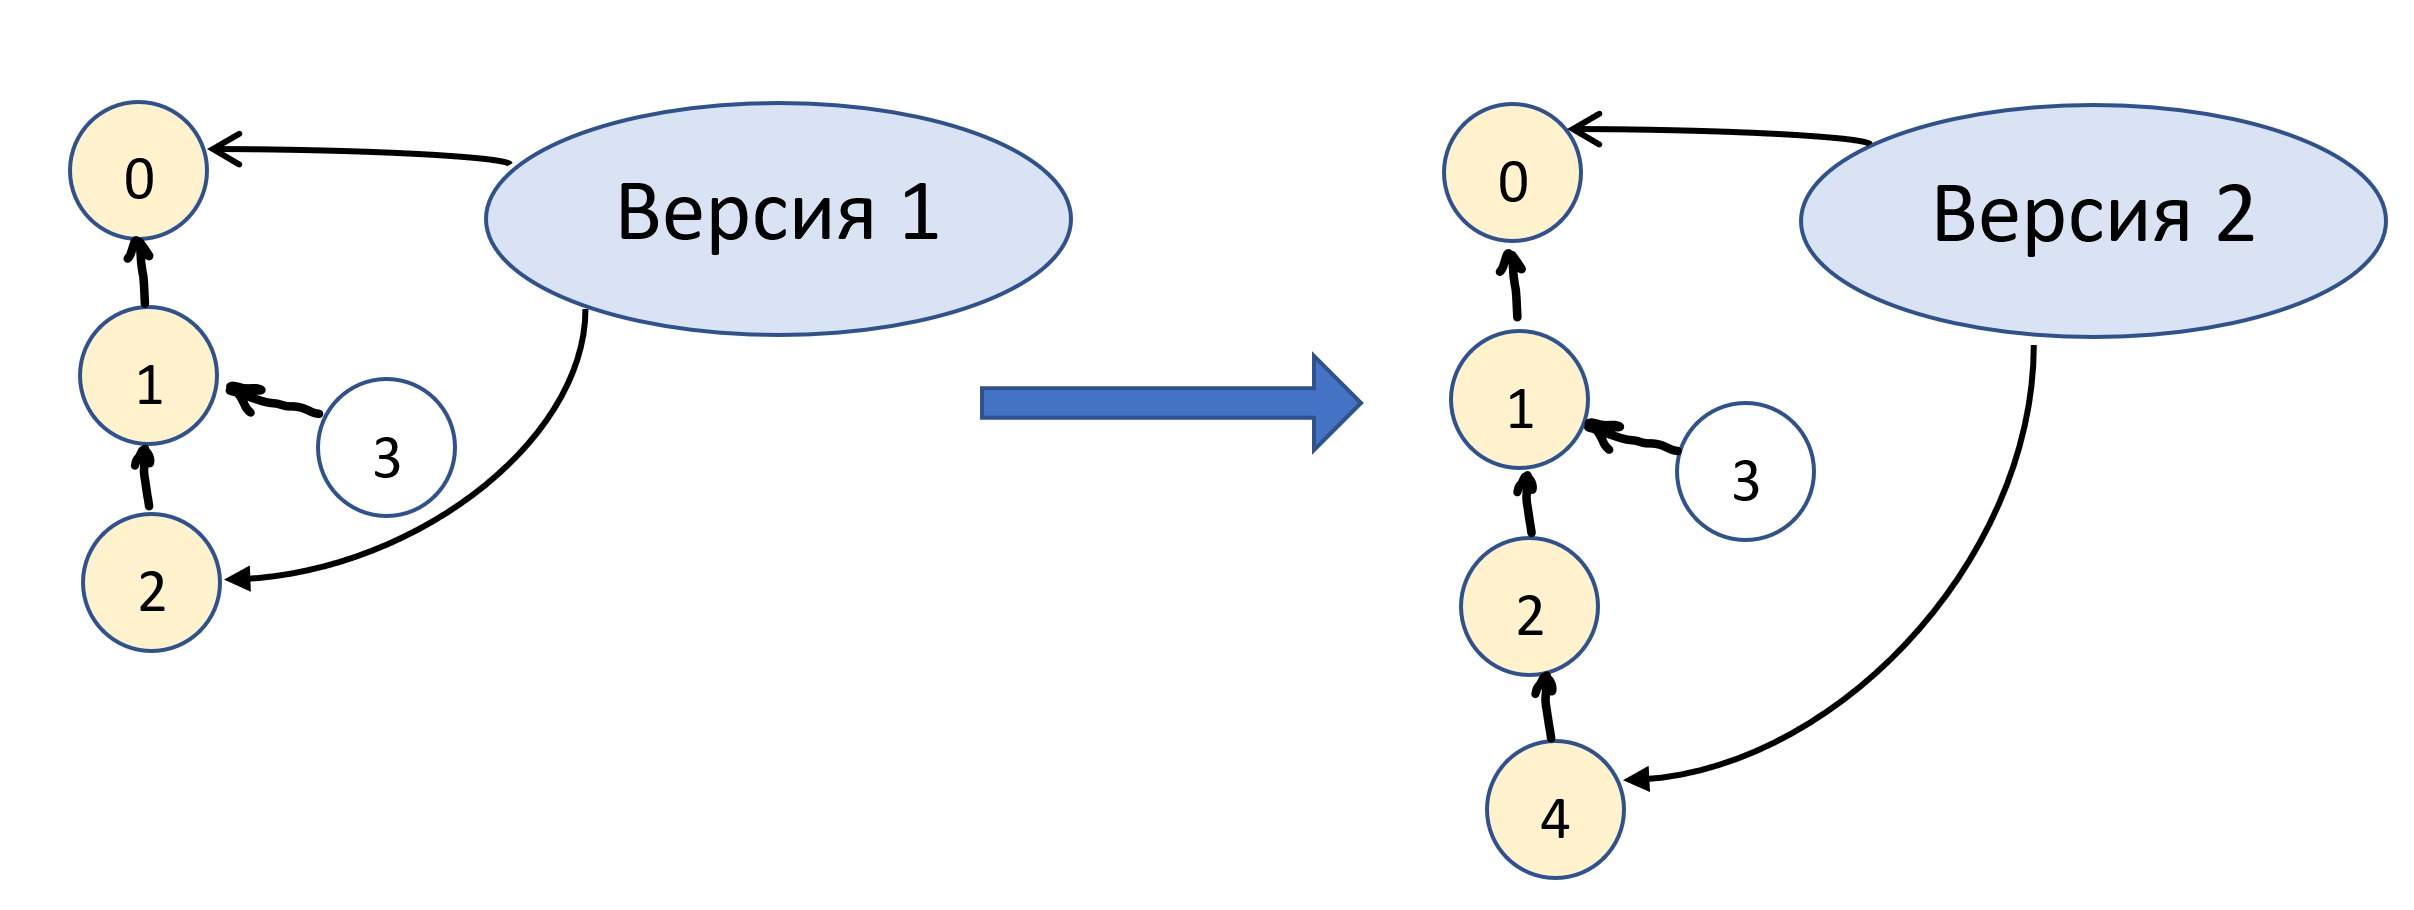
\includegraphics[width=0.9\textwidth]{content/2_img.jpg}
	\caption{Добавление вершины произвести легко}
	\label{insertion}
\end{figure}\par
Однако, при операции Удаления возникнет проблема — из-за односвязности списков, мы не можем за константное время узнать, какая вершина станет следующей головой, так как для этого нам придется последовательно пройти по указателям от хвостовой вершины до вершины, предшествующей голове, чтобы узнать указатель на нее. Это может привести время выполнение операции к асимптотике $O(n)$, где $n$ — количество элементов в выбранной очереди.\par
Чтобы избежать такой проблемы, добавим понятие вспомогательных списков Версии и модифицируем объекты Версий следующим образом: добавим в объект Версии указатель на такой список, что его хвостовой элемент хранит в себе указатель на вершину, следующую за головой Версии, следующий элемент — на третью вершину с начала и так далее (то есть список из промежуточных вершин очереди, развернутый в обратную сторону). Таким образом, мы будем знать, какая вершина следует за головой — достаточно просто посмотреть, на какую вершину Основного дерева указывает ведущая вершина вспомогательного списка.\par
Однако, на этом месте возникает новая проблема — как строить такой вспомогательный список? Мы не можем строить заново список промежуточных вершин на каждом шаге (иначе это приведет нас к старой асимптотике). Решим это добавлением в объект Версии, помимо указателя на вспомогательный список, нового указателя на строящийся вспомогательный список. Для удобства, существующий вспомогательный список будем называть Операционным, строящийся — Динамическим. Оба эти списка по своей природе являются продолжениями друг друга, поэтому их можно хранить в одном Вспомогательном дереве.\par
После совершения какой либо операции над Версией, будем проверять, есть ли динамический список у этой Версии.\par
Если его нет, то проверяем, не надо ли начать строить его (критерий проверки и его корректность будут приведены в следующем разделе). Если такой необходимости нет, то можно заканчивать выполнение операции. Иначе, создаем вспомогательную вершину, в которой указатель на сына оставляем нулевым, а в указатель на целевую вершину записываем указатель на сына хвостовой вершины.\par
После этого проверяем, не надо ли поменять списки местами — для этого достаточно сделать проверку, что сын целевой вершины ведущей вершины динамического списка — голова Версии. Если это так, то подменяем указатель Версии на операционный список указателем на динамический, а указатель на динамический список — зануляем.\par
Если же динамический список уже начал строиться, то на каждой операции просто будем достраивать его. Но перед этим необходимо проверить, нельзя ли поменять операционный и динамический списки местами. Если поменять их удалось, то на этом выполнение операции прекращается. Иначе, создаем вспомогательную вершину, в которой указатель на сына выставляем на ведущую вершину динамического списка исходной Версии, а в указатель на целевую вершину записываем указатель на сына целевой вершины ведущей вершины динамического списка исходной версии. Снова делаем попытку смены списков друг на друга.\par
Тогда, операция Удаления будет проходить следующим образом:\\
Если размер очереди $1$, то достаточно скопировать нулевую Версию в конец списка (созданная версия будет пуста, то есть эквивалентна изначальной).\\
Если размер очереди $2$, то достаточно в новой Версии в указатель на голову записать указатель Версии на хвост.\\
Иначе, если размер $> 2$, в указатель на голову новой Версии записываем указатель на целевую вершину ведущей вершины операционного списка Версии. В указатель на операционный список Версии записываем указатель на сына ведущей операционной вершины Версии. При необходимости достраиваем динамический список.\par
Таким образом, удаление вершины и возможное достраивание динамического списка происходят за константное время, как и результирующая операция Удаления, что и хотели получить.

\subsection{Критерий построения динамического списка}
Для определения необходимости начала построения динамического списка будем пользоваться следующим условием:\\
\emph{Если длина операционного списка $< \frac{1}{2}$ от количества промежуточных вершин очереди, то необходимо начать строить динамический список.}\par
Покажем, почему выполнение данного критерия позволяет всегда поддерживать знание о том, какая вершина следует за головой очереди и не произойдет ситуации, когда операционный список уже закончился, а динамический не успел достроиться до головы. Для этого докажем, что для любой Версии поддерживается уравнение
\begin{equation}
    \label{equ}
        2p + d = r,
\end{equation}
где $p$ и $d$ - количество вершин в операционном и динамическом списках соответственно, а $r$ - количество промежуточных вершин очереди. Доказательство по матиндукции:\\
База:\\
На первом шаге, когда мы начинаем конструирование динамического списка, в нем находится одна вершина, то есть $d_{new} = 1$. Для текущей очереди выполняется $2p_{new} - r_{new} < 0$, для ее родительской Версии выполняется $2p_{old} - r_{old} \geqslant 0$, так как на предыдущем шаге критерий еще не был выполнен и динамический список не начинал строиться. Рассмотрим два возможных варианта:\\
1. Пусть для получения новой Версии была использована операция Добавления. В таком случае, $p_{new} = p_{old}$ (операционный список в данном случае не менялся), $r_{old} + 1 = r_{new}$ (добавление вершины в очередь увеличивает количество промежуточных). Тогда, получаем
\begin{equation}
    \nonumber2p_{new} - r_{new} = 2p_{old} - (r_{old} + 1) \Rightarrow 2p_{new} - r_{new} + 1 = 2p_{old} - r_{old} = 0,
\end{equation}
то есть $2p_{new} + 1 = r_{new}$, что совпадает с условием $d_{new} = 1$.\\
2. Пусть для получения новой Версии была использована операция Удаления. В таком случае, $p_{new} = p_{old} - 1$, (операционный список в данном случае уменьшился на 1 из-за перехода), $r_{new} = r_{old} - 1$ (удаление вершины из очереди уменьшает количество промежуточных). Тогда, получаем
\begin{equation}
    \nonumber2p_{new} - r_{new} = 2(p_{old} - 1) - (r_{old} - 1) = 2p_{old} - r_{old} - 1 \Rightarrow 2p_{new} - r_{new} + 1 = 2p_{old} - r_{old} = 0,
\end{equation}
то есть $2p_{new} + 1 = r_{new}$, что совпадает с условием $d_{new} = 1$.\\
База доказана.\\
Переход:\\
Пусть это равенство выполняется для какого-то шага алгоритма, когда динамический список уже есть. Рассмотрим случаи:\\
Пусть для получения новой Версии была использована операция Добавления. В таком случае, $p_{old} = p_{new}$ (операционный список в данном случае не менялся), $r_{old} = r_{new} - 1$ (добавление вершины в очередь увеличивает количество промежуточных). Тогда, получаем
\begin{equation}
    \nonumber2p_{old} - r_{old} = 2p_{new} - (r_{new} - 1) \Rightarrow 2p_{old} - r_{old} = 2p_{new} - r_{new} + 1,
\end{equation}
то есть $d_{old} + 1 = d_{new}$, что и достигается добавлением динамической вершины в алгоритме.\\
Пусть для получения новой Версии была использована операция Удаления. В таком случае, $p_{old} = p_{new} + 1$, (операционный список в данном случае уменьшился на 1 из-за перехода), $r_{old} = r_{new} + 1$ (удаление вершины из очереди уменьшает количество промежуточных). Тогда, получаем
\begin{equation}
    \nonumber2p_{old} - r_{old} = 2(p_{new} + 1) - (r_{new} + 1) = 2p_{new} - r_{new} + 1,
\end{equation}
то есть $d_{old} + 1 = d_{new}$,что и достигается добавлением динамической вершины в алгоритме.\\
Переход доказан.\\
Так как проблемы могут возникнуть только при операции Удаления (вспомогательные списки используются только для нее), то докажем от противного для этой ситуции. Пусть мы хотим совершить операцию Удаления, но у нас нет операционного списка. Тогда, возможны 2 случая:
\begin{enumerate}
    \item Динамический список не был построен для данной Версии.
    \item Динамический список не успел достроиться до головы очереди.
\end{enumerate}\par
В первом случае, если динамический список не начинал строиться, то выполняется $2p \geqslant r$, но $p = 0 \Rightarrow r = 0 \Rightarrow$ в очереди нет промежуточных вершин, то есть размер очереди $\in [0, 2]$, но в таком случае нам не нужен операционный список, так как для очередей размера $\leqslant 2$ операция Удаления не задействует вспомогательные списки.\par
Во втором случае, динамический список имеет ненулевой размер. Воспользуемся полученным равенством~(\ref{equ}) и применим его, тогда в силу $p = 0$ получаем $d = r$, но это означает, что динамический список был достроен до головы и должен был подменить операционный еще на предыдущем шаге.\\
Таким образом, приведенная по условию ситуация при Удалении невозможна.\par
Последним шагом покажем, что при достижении головы очереди на момент подмены операционного списка динамическим, его длина $2d \geqslant r$, то есть не возникнет ситуации, что построенный новый операционный список будет слишком коротким и построение следующего динамического списка запоздает. $2d \geqslant r \Leftrightarrow d \geqslant r - d$, а это число является количеством промежуточных вершин, не содержащихся на данный момент в динамическом списке. Так как промежуточные вершины возникают только при выполнении операции Добавления, а динамический список будет пополняться на каждом шаге, то несложно понять, что неравенство выполняется, то есть при обмене операционного списка на динамический будет гарантирована его необходимая длина.\\
То есть применение данного критерия в алгоритме корректно.

\pagebreak
\subsection{Итоговая версия алгоритма}
\noindentПриведем полученную нами итоговую версию алгоритма:
\begin{figure}[h!]
	\centering
	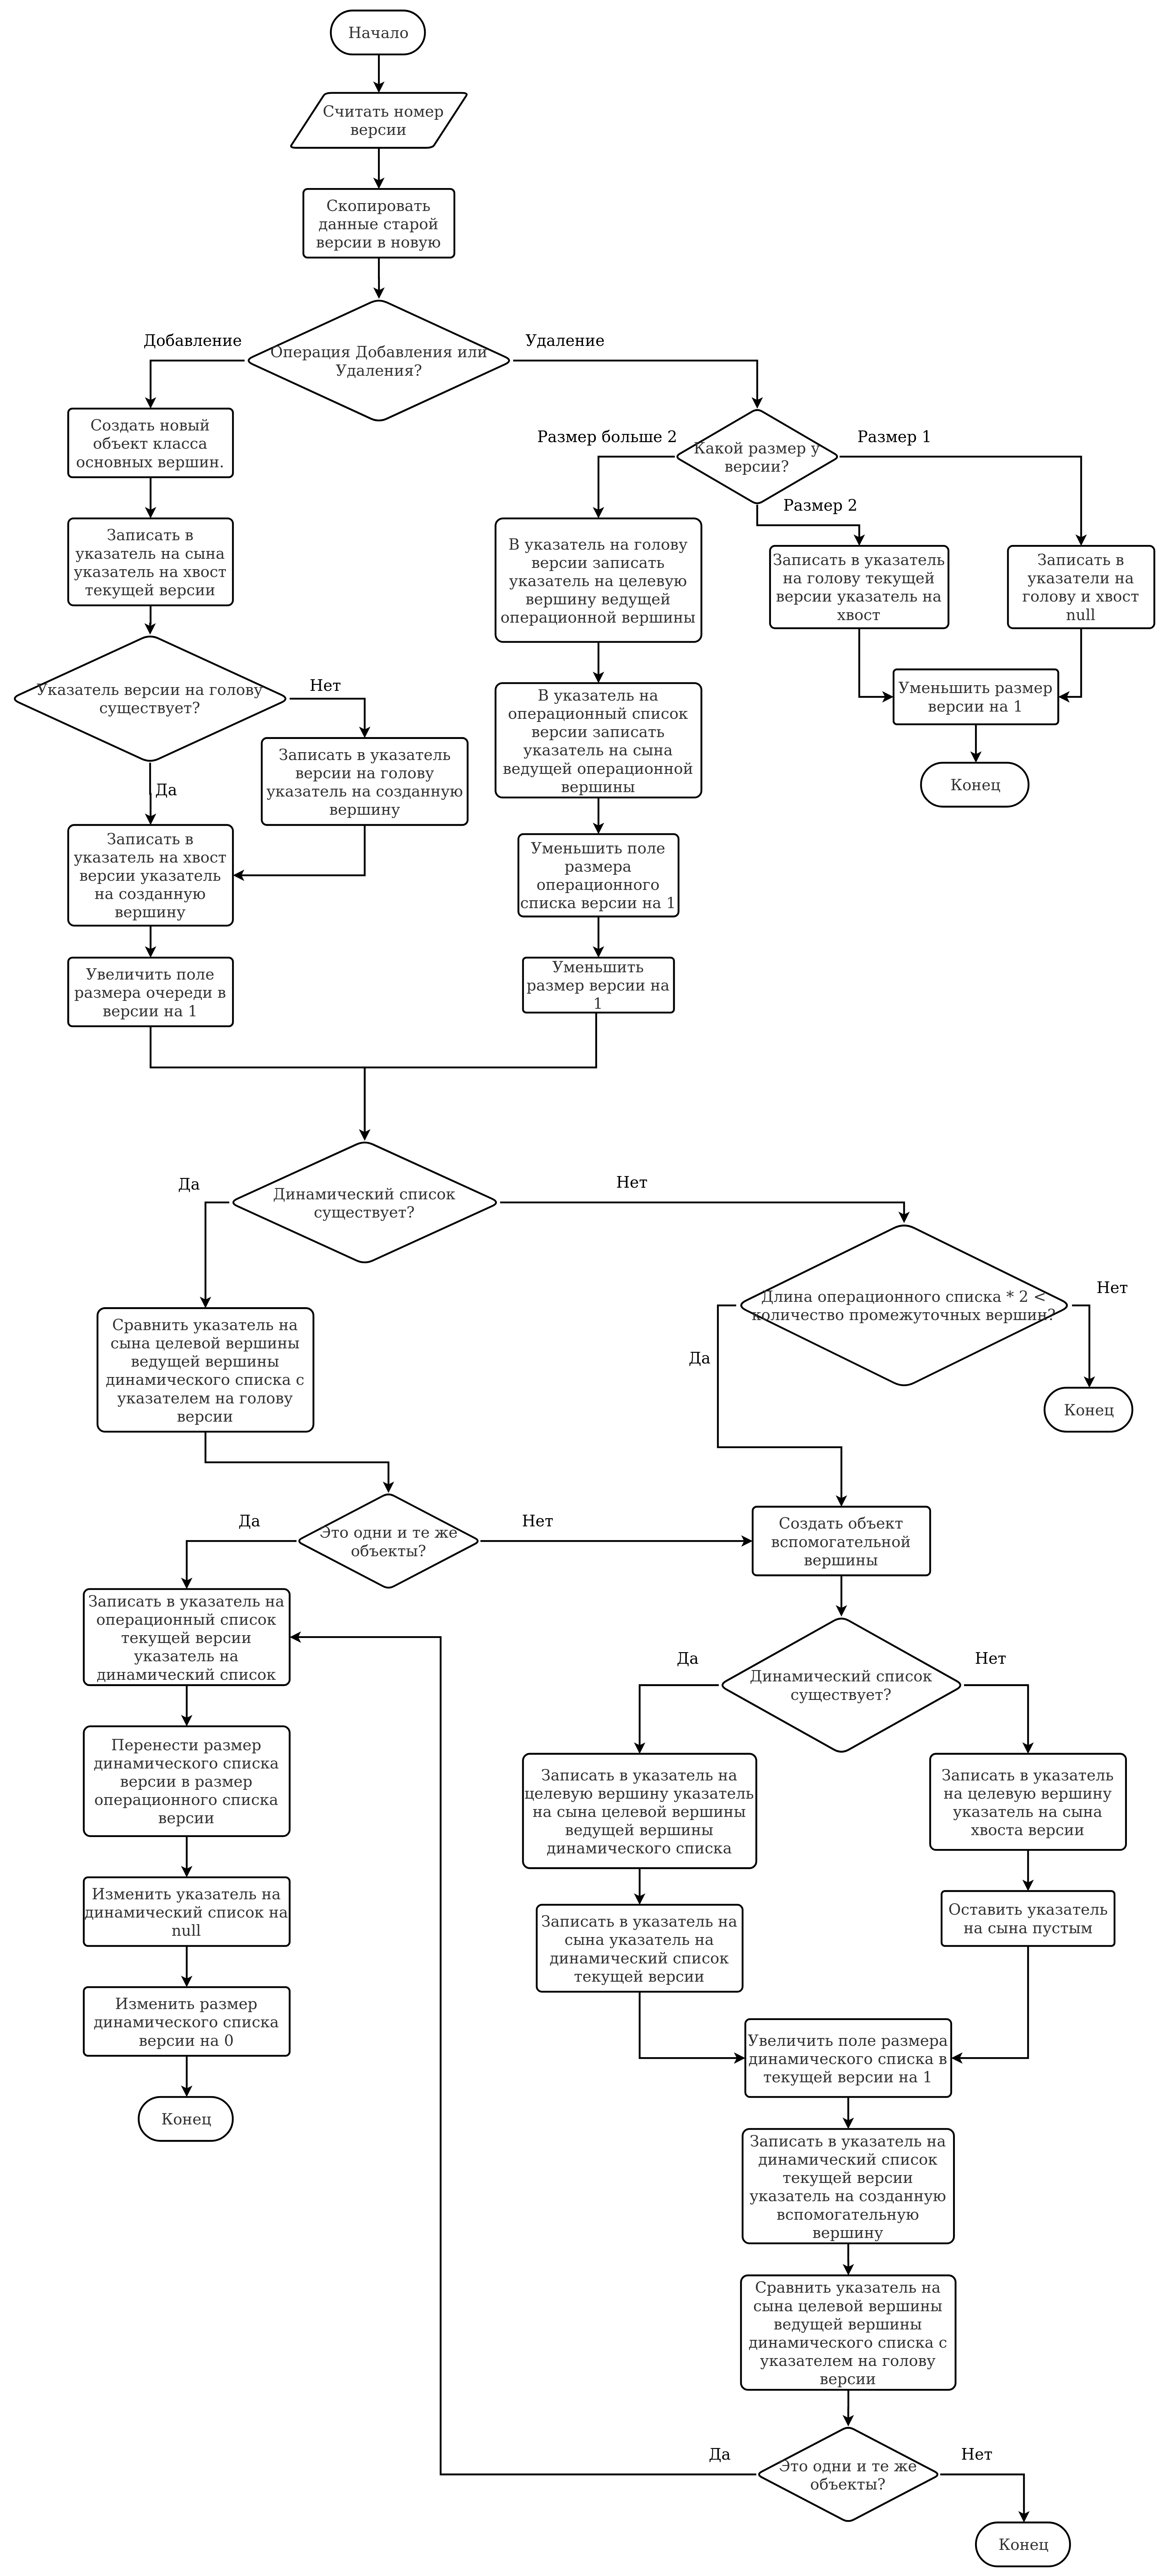
\includegraphics[width=0.58\textwidth]{content/Persistent queue algorithm flowchart.png}
	\caption{Общая блок-схема работы алгоритма}
	\label{block-scheme}
\end{figure}
\pagebreak

\subsection{Код алгоритма на С++}
\noindentПриведем полученный возможный код алгоритма на языке C++:
\begin{lstlisting}
#include "vector"

struct QueueNode {
    QueueNode *son;
    int64_t value;
};

struct ListNode {
    ListNode *next_list;
    QueueNode *target_node;
    int64_t size;
};

struct Version {
    QueueNode *head;
    QueueNode *tail;
    ListNode *operational_list;
    ListNode *dynamic_list;
    int64_t size;
};

class PersistentQueue {
public:
    explicit PersistentQueue(int64_t num_of_actions) {
        versions.reserve(num_of_actions + 2);
        versions.push_back(new Version({nullptr, nullptr, nullptr, nullptr, 0}));
    }

    void Push(int64_t parent_queue_num, int64_t value_to_push) {
        Version *parent = versions[parent_queue_num];
        auto *new_node = new QueueNode({parent->tail, value_to_push});
        QueueNode *first_el = parent->size ? parent->head : new_node;
        versions.push_back(new Version({first_el,
                                        new_node,
                                        parent->operational_list,
                                        parent->dynamic_list,
                                        parent->size + 1}));
        ChangeDynamicList();
    }

    void Pop(int64_t parent_queue_num) {
        Version *parent = versions[parent_queue_num];
        if (parent->size == 1) {
            versions.push_back(new Version({nullptr,
                                            nullptr,
                                            nullptr,
                                            nullptr,
                                            0}));
        } else if (parent->size == 2) {
            versions.push_back(new Version({parent->tail,
                                            parent->tail,
                                            nullptr,
                                            nullptr,
                                            1}));
        } else {
            versions.push_back(new Version({parent->operational_list->target_node,
                                            parent->tail,
                                            parent->operational_list->next_list,
                                            parent->dynamic_list,
                                            parent->size - 1}));
            ChangeDynamicList();
        }
    }

private:
    void ChangeDynamicList() {
        Version *current = versions[versions.size() - 1];
        if (current->dynamic_list) {
            if (!ListsExchange()) {
                QueueNode *new_dynamic_node =
                        current->dynamic_list->target_node->son;
                int64_t new_size = current->dynamic_list->size + 1;
                current->dynamic_list = new ListNode({current->dynamic_list,
                                                      new_dynamic_node,
                                                      new_size});
                ListsExchange();
            }
            return;
        }
        int64_t operational_list_size = current->operational_list ?
                                        current->operational_list->size
                                        : 0;
        int64_t curr_version_nodes_size = std::max(NULL, current->size - 2);
        if (operational_list_size * 2 < curr_version_nodes_size) {
            QueueNode *new_dynamic_node = current->tail->son;
            current->dynamic_list = new ListNode({nullptr,
                                                  new_dynamic_node,
                                                  1});
            ListsExchange();
        }
    }

    bool ListsExchange() {
        Version *current = versions[versions.size() - 1];
        if (current->dynamic_list->target_node->son == current->head) {
            current->operational_list = current->dynamic_list;
            current->dynamic_list = nullptr;
            return true;
        }
        return false;
    }

    std::vector<Version *> versions;
};
\end{lstlisting}

\subsection{Оценка производительности}
Каждая операция выполняется за константное время (что видно из блок-схемы), кроме копирования Версии в конец их списка. Так как нам необходим произвольный доступ к различным элементам этого списка, самым оптимальным решением будет обычный массив, в который вставка происходит за $O(1)$ амортизированное. Таким образом, итоговая оценка сложности по времени выполнения всех операций — $O(1)$ амортизированное.\par
На каждую операцию создается новый объект Версии, а так же добавляются вершины в граф. В худшем случае, на каждую операцию будет создаваться как обычная вершина очереди, так и новая вспомогательная для динамического списка, что в итоге приводит к сложности алгоритма по памяти $O(3n) \sim O(n)$. Приведем результаты сравнения работы предложенного алгоритма с другими распространенными вариантами:
\begin{table}[ht]
	\label{algo_times}
	\footnotesize
	\centering
	\begin{tabular}{сrrrrrrrr}
		\toprule
		& \multicolumn{3}{c}{Время работы} &
		\multicolumn{3}{c}{Затраченная память} \\
		\cmidrule(lr){2-4} \cmidrule(l){5-7} 
		{} &  {Макс.} &  {Среднее} &  {Медианное} &  {Макс.} &  {Среднее} &  {Медианное}\\
		\midrule
		\begin{tabular}{@{}c@{}}Персистентное \\ дерево отрезков\end{tabular} & 367ms & 214ms & 210ms & 197.7Mb & 102.4Mb & 75.7Mb\\
		\begin{tabular}{@{}c@{}}Персистентное\\декартово дерево\\по неявному ключу\end{tabular} & 351ms & 197ms & 201ms & 135.2Mb & 87.3Mb & 61.9Mb\\
		\begin{tabular}{@{}c@{}}Алгоритм на\\6 стеках\end{tabular} & 230ms & 139ms & 131ms & 57.7Mb & 34.3Mb & 38.1Mb\\
        \begin{tabular}{@{}c@{}}Мой\\алгоритм\end{tabular} & 99ms & 69ms & 87ms & 19.5Mb & 13.7Mb & 18.0Mb\\
		\midrule
		\bf{\begin{tabular}{@{}c@{}}Отличие от \\лучшего значения\end{tabular}} & \bf{131ms} & \bf{70ms} & \bf{44ms} & \bf{38.2Mb} & \bf{20.6Mb} & \bf{20.1Mb} \\
		\bottomrule
	\end{tabular}
    \caption{Статистика работы различных алгоритмов обработки Персистентной очереди на одном и том же наборе данных}
\end{table}

\section{Разработка веб-приложения}
\noindentПосле выбора алгоритма, на котором будет строиться объяснение и визуализация, появилась возможность перейти к разработке самого веб-приложения. Условно можно разбить всю его реализацию на несколько частей:
\begin{enumerate}
    \item Поиск и изучение библиотеки для визулизации графов.
    \item Перенос алгоритма на JavaScript с добавлением необходимых данных для подробной визуализации внутренней работы.
    \item Добавление инструментов визуальной помощи в объяснении шагов алгоритма.
    \item Добавление интерфейса взаимодействия с HTML-страницей.
    \item Стилизация элементов с помощью CSS.
    \item Реализация дополнительных возможностей для пользователя.
\end{enumerate}

\subsection{Библиотека для визулизации графа}
Для реализации динамических анимаций с графами мне была необходима библиотека, способная работать с такими данными. Из разных вариантов больше всего мне подошла библиотека D3~\cite{d3}, которая дает широкий выбор возможностей и удобный программный интерфейс взаимодействия (по сравнению со своими аналогами, например Cytoscape).\par
После этого, мне было необходимо изучить способы отображения графов, их симуляцию, поведение и какие данные необходимы для их корректного отображения. Мне был необходим стиль визуализации force-directed graph layout — способ рисовки графа, в котором поддерживаются связи между вершинами, при этом каждая вершина имеет отрицательный коэффициент притяжения (отталкивается от других), а каждое ребро имеет положительный коэффициент (притягивает соединенные вершины друг к другу). Таким образом, граф сохраняет целостность и не происходит наложение вершин, либо пересечение ребер друг с другом.\par
Также, любая перестройка графа сопровождается определенным периодом симуляции его обновления. В течение этого времени силы притяжения активны и под их влиянием граф может видоизменяться. Традиционно, параметр отвечающий за время перестройки изменяется по принципу отжига. После того, как этот параметр достигнет определенного уровня, перестройка завершается и положение графа фиксируется.

\subsection{Перенос алгоритма на JavaScript}
Так как JavaScript не имеет возможностей прямых манипуляций с памятью, то реализовать алгоритм полностью в исходном виде не получится. По этой причине все структуры, которые предполагали хранение в памяти и адресацию по указателям, будут храниться в обычных массивах и в качестве адресации использовать индексы, по которым эти элементы можно найти. Это решение незначительно влияет на скорость работы, так как операции с массивами происходят за амортизированно константное время. Таким образом, интерфейс классов объектов Версий и вершин Основного и Вспомогательного деревьев логически не изменился, по сравнению с исходной реализацией.\par
Но так как визуализация должна поддерживать пошаговость, необходимо добавить остановки после каждого действия, чтобы дать пользователю возможность контролировать ход выполнения алгоритма. Также требуется реализовать и откаты назад по шагам алгоритма, что будет сложно сделать в рамках одной функции на программном уровне, поэтому был реализован следующий механизм работы:\\
Все функции разбиты на цепочные — каждая из функций возвращает указатель на следующую функцию для вызова.\\
На вызове каждой операции, запускается координатор выполнения этих функций. После выполнения каждой из них, в зависимости от решения пользователя, он либо продолжает вызовы следующих функций, либо производит откат назад с восстановлением параметров.\\
Для восстановления состояния окружения на момент вызова каждой из функций, был реализован класс Состояний, который перед вызовом любой функции производит копирование необходимых параметров и аргументов вызова, если таковые имелись. В случае, когда происходит откат назад, в переменные загружаются сохраненные значения и происходит повторный вызов функции с сохраненными аргументами.

\subsection{Инструменты помощи в объяснении шагов}
Для большей наглядности требуется каждый шаг сопровождать подсказками для пользователя. Это облегчает понимание алгоритма и его ход работы, при этом позволяет не изучать его техническую работу в деталях. С этой целью были созданы следующие инструменты:\\
Подсветка Версий — такая подсветка выделяет соответствующую выбранной Версии очередь и ее вспомогательные списки, при этом затемняя элементы, не относящиеся к данной Версии.\\
Подсветка вершин и ребер — если на каком-либо шаге алгоритма происходит изменение графа, либо же производится переход и поиск данных в вершинах, то они визуально выделяются, для подчеркивания с какой именно вершиной/ребром идет работа в данный момент.\\
Внутренняя информация объектов — при наведении на различные объекты (Версии, вершины основного и вспомогательного деревьев) выдается внутренняя информация, которую хранят данные объекты. Для Версий это "указатели" на начало, конец очереди, а также на вспомогательные списки. Для вершин это их сыновья, для вспомогательных вершин дополнительно показываются целевые вершины в Основном графе.\\
Текстовое сопровождение — на каждом шаге добавлено текстовое объяснение текущего шага и логика его работы, позволяющее проследить цепочку логического выполнения алгоритма.

\subsection{Взаимодействие с HTML-страницей}
Для видоизменения страницы разработан интерфейс взаимодествия с ней. При определенных операциях убираются лишние объекты, либо наоборот возвращаются.\\
Также сделана система перевода элементов на разные языки — для этого достаточно только загрузить необходимый .json файл с объявлениями переводов элементов, после чего страница может быть переведена на этот язык. Добавленный язык можно выбрать из меню приложения, где с этой целью создан выпадающий список доступных переводов.\\
Чтобы добавить возможность совершения различных операций, добавлены соответствующие кнопки и поля для заполнения.\\
Дополнительные файлы для отображения на странице, такие как картинки, могут быть добавлены из соответствующей папки.

\subsection{Дополнительные возможности}
Для удобства пользователя создана инструкция, в которой полностью описан интерфейс приложения и способы взаимодействия с ним.\
Создан сборник готовых наборов данных, которые выполняют определенные операции, наглядно демонстрирующие различные поведения алгоритма.\\
Пользователь может также создать случайный граф очередей, задав некоторые параметры его создания (например, размер или характер создания).\\
Есть возможность переключения между режимами работы — пошаговой работой алгоритма и мгновенным выполнением всех операций.\\
Дополнительные незначительные функции, вроде удаления всех данных приложения или обновления визуализации графов.

\section{Заключение}
В результате проведенной работы было получено полностью работоспособное приложение, которое может выполнять все заложенные в него требования. Из-за специфики темы и выбора алгоритма, на данный момент нет каких-либо аналогов данного приложения, либо его возможных альтернатив на других алгоритмах. В дальнейшем, данное веб-приложение может поддерживаться и обновляться, так как создана базовая система, в которую можно добавлять улучшения без больших затрат по времени.

\subsection{Возможные улучшения и оптимизации алгоритма}
В данном алгоритме есть возможность уменьшения использования дополнительной памяти, в нескольких случаях:\par
Если выполннить две операции Добавления к одной и той же Версии, то если выполняется критерий построения динамического списка (либо список уже начат), во Вспомогательный граф будут добавлены две абсолютно идентичные вершины. В таком случае, можно было бы создать вспомогательную вершину только для первой операции, а для второй — обратиться к уже существующей. Это может сильно уменьшить потребление памяти при выполнении множества операций, примененных к узкому набору Версий.\par
Если последовательно выполнять операции Добавления к Версии, у которой уже есть операционный список, то в динамический список с какого то момента будут добавляться вершины, которые уже есть в операционном списке (это происходит из-за того, что динамический список стремится пройти до головной вершины Версии, а не последней вершины операционного списка). Добавив дополнительную информацию в объект Версии о том, какая вершина завершает операционный список, можно сильно уменьшить потребление памяти при последовательных монотонных операциях.\par
Однако, в силу того, что обе эти оптимизации требуют либо дополнительной структуры данных о существующих связях (первая оптимизация), либо дополнительных полей в объектах (вторая оптимизация), то их результативность неоднозначна и должна применяться в соответствии со спецификой требований от алгоритма. Где-то требуются множественные изменения к нескольким Версиям, а где-то — изменения последовательно применяются к цепочке Версий. В зависимости от варианта работы, будет целесообразно реализовать ту или иную оптимизацию.

\subsection{Возможные улучшения веб-приложения}
На данный момент приложение визуализирует только хранение по одному алгоритму. Если подготовить новые алгоритмы и их визуальное сопровождение, то будет несложно интегрировать их в существующую систему. При наличии нескольких алгоритмов, можно создать возможность для пользователя строить графы на больших объемах данных и сравнивать технические характеристики алгоритмов (такие как потребление памяти, затраченное время на исполнение и так далее).\\

\newpage 
\printbibliography[heading=bibintoc]
\end{document}